\documentclass[10pt,a4paper]{article}

\usepackage[utf8]{inputenc}
\usepackage[T1]{fontenc}
\usepackage[spanish, es-tabla]{babel}
\usepackage{lmodern}
\usepackage{csquotes}
\usepackage{amsmath, amsfonts, amssymb, amsthm}
\usepackage{graphicx}
\usepackage{subcaption}
\usepackage{float}

\usepackage[
    left=2.54cm,
    right=2.54cm,
    top=2.54cm,
    bottom=2.54cm
]{geometry}

\usepackage{tikz}
\usepackage{soul}
\usepackage{listings}
\usepackage[most]{tcolorbox}
\usepackage{xcolor}
\usepackage{hyperref}

\tcbset{shield externalize}

\usetikzlibrary{arrows.meta, positioning, automata}
\usetikzlibrary{babel}
\usetikzlibrary{external}

\tikzexternalize[prefix=build-tikz/]



\lstset{
    basicstyle=\footnotesize\ttfamily,
    frame=single,
    numbers=left,
    inputencoding=utf8,
    extendedchars=true,
    breaklines=true,
    showstringspaces=false,
    keywordstyle=\color{blue},
    commentstyle=\color{green!50!black},
    stringstyle=\color{red!70!black}
}


\newtcbtheorem[number within=section]{ejercicio}{Ejercicio}{
    enhanced,
    sharp corners,
    boxrule=0pt,
    leftrule=5pt,
    colframe=gray!30!black,
    colback=gray!5!white,
    coltitle=white,
    fonttitle=\bfseries,
    separator sign={.\ },
    before skip=10pt,
    after skip=10pt
}{ej}



\newtcbtheorem[number within=section]{mytheo}{Teorema}{
    enhanced,
    sharp corners,
    boxrule=0pt,
    leftrule=5pt,
    colframe=blue!40!black,
    colback=blue!5!white,
    coltitle=white,
    fonttitle=\bfseries,
    separator sign={.\ },
    before skip=10pt,
    after skip=10pt
}{th}



\newtcolorbox{alerta}[1]{
    enhanced,
    sharp corners,
    boxrule=0pt,
    leftrule=5pt,
    colframe=red!40!black,
    colback=red!5!white,
    coltitle=white,
    fonttitle=\bfseries,
    title=#1,
    before skip=10pt,
    after skip=10pt
}

\newtcolorbox{nota}[1]{
    enhanced,
    sharp corners,
    boxrule=0pt,
    leftrule=5pt,
    colframe=orange!40!black,
    colback=yellow!5!white,
    coltitle=white,
    fonttitle=\bfseries,
    title=#1,
    before skip=10pt,
    after skip=10pt
}


\begin{document}


\begin{titlepage}

    \centering

    {\huge \textbf{Universidad Nacional Autónoma de México}}\\[0.3cm]

    \rule{\linewidth}{2mm}\\[0.3cm]

    {\large \textbf{Facultad de Estudios Superiores Acatlán}}\\[1cm]

    
\includegraphics[width=6cm]{../../../../Archivos/Imagenes_Logos/acatlan.png}\\[1cm]

    {\Large \textbf{Matemáticas Aplicadas y Computación}}\\[1cm]

    {\huge \textbf{Database Administrator}}\\[0.5cm]

    \rule{\linewidth}{1mm}\\[0.3cm]

    \vfill

    {\Large \textit{Movilidad Urbana: Análisis del Sistema Ecobici en la CDMX.}\\[0.5cm]}

    \vfill

    {\Large \textit{Equipo 6.}}\\

    \rule{\linewidth}{0.5mm}\\[0.3cm]

    {\Large \textit{López Ramírez Ricardo.}}\\
    {\Large \textit{Ruiz Sánchez Emiliano}}\\
    {\Large \textit{Cabrera Trejo José Luis}}\\
    {\Large \textit{Estrada Romero Meliza Edith}}\\

    \rule{\linewidth}{0.5mm}\\[0.8cm]

    \small

    Actualización: \today

\end{titlepage}



\pagenumbering{roman}

\tableofcontents

\clearpage

\pagenumbering{arabic}

\setcounter{page}{1}


\section{Tema y Descripción del Proyecto}

\subsection{Descripción General}
\textbf{Movilidad Urbana: Análisis del Sistema Ecobici en la Ciudad de México}, 
consiste en el diseño, estructuración e implementación de una base de datos relacional 
analítica enfocada en la red de transporte de bicicletas de la CDMX. A través de la 
aplicación de técnicas de Inteligencia de Negocios (BI) y un diseño de arquitectura basada en 
un Modelo de Estrella, el proyecto procesa y normaliza un volumen masivo de datos transaccionales 
correspondientes a los años 2024, 2025 y 2026. 

\subsection{Elección del Tema}
Se seleccionó este tema porque el sistema Ecobici es fundamental de la movilidad sustentable y el desarrollo
urbano inteligente en la capital del país. Desde una perspectiva de ingeniería de datos, 
el sistema genera un volumen de información masivo diariamente. 
Esto nos presentó un escenario ideal, altamente retador y apegado a la realidad de la industria, 
para aplicar técnicas avanzadas de administración de bases de datos. 
Resolver las limitantes de particionamiento del motor de bases de datos mientras se garantizaba un 
100\% de integridad referencial, demuestra el nivel técnico requerido para gestionar 
arquitecturas de datos.

\subsection{Información a Visualizar en la Base de Datos}
La base de datos está estructurada para visualizar la interacción entre los usuarios y el sistema de movilidad mediante las siguientes dimensiones y métricas:
\begin{itemize}
    \item \textbf{Hechos de Movilidad:} Más de 6.5 millones de registros operativos en la tabla principal y más de 30 millones en el histórico, detallando cada viaje realizado.
    \item \textbf{Perfiles Demográficos:} Género y edad de los usuarios, permitiendo segmentar el comportamiento del consumidor.
    \item \textbf{Dimensión Espacial:} Catálogo de estaciones de retiro y arribo, incluyendo su nomenclatura y zonificación, para trazar las rutas urbanas.
    \item \textbf{Dimensión Temporal:} Fechas exactas y franjas horarias (Mañana, Tarde, Noche, Madrugada) para identificar horas pico y valles de demanda.
    \item \textbf{Inventario Físico:} Estatus y tipo de las bicicletas utilizadas.
\end{itemize}


\begin{table}[h]
\centering
\caption{Volumetría de Datos del Proyecto}
\vspace{0.2cm}
\begin{tabular}{|l|c|l|}
\hline
\textbf{Tabla / Entidad} & \textbf{Tipo en Modelo} & \textbf{Volumen Aproximado} \\ \hline
Historico Viajes & Tabla Particionada & $> 30,000,000$ registros \\ \hline
Viajes (2025-2026) & Tabla de Hechos & $> 6,500,000$ registros \\ \hline
Estaciones & Catálogo / Dimensión & 683 estaciones únicas \\ \hline
Tiempos & Dimensión Temporal & 86,400 segundos \\ \hline
\end{tabular}
\label{tab:volumetria}
\end{table}

\subsection{Finalidad Principal}
La finalidad principal de esta base de datos no es únicamente el almacenamiento, servir  
como un repositorio analítico robusto. El objetivo es transformar los datos crudos en 
información estratégica que permita a los tomadores de decisiones optimizar la logística del sistema. 
Mediante las sentencias DML avanzadas desarrolladas en el proyecto, la base de datos es capaz de responder 
preguntas de negocio complejas en segundos, tales como: la saturación de las estaciones por franjas horarias, 
los patrones de ruta más frecuentes según el género del usuario, y la proyección de mantenimiento del inventario 
de bicicletas.

\newpage

\section{Diagrama Entidad-Relación}

\begin{figure}[h]
    \centering
    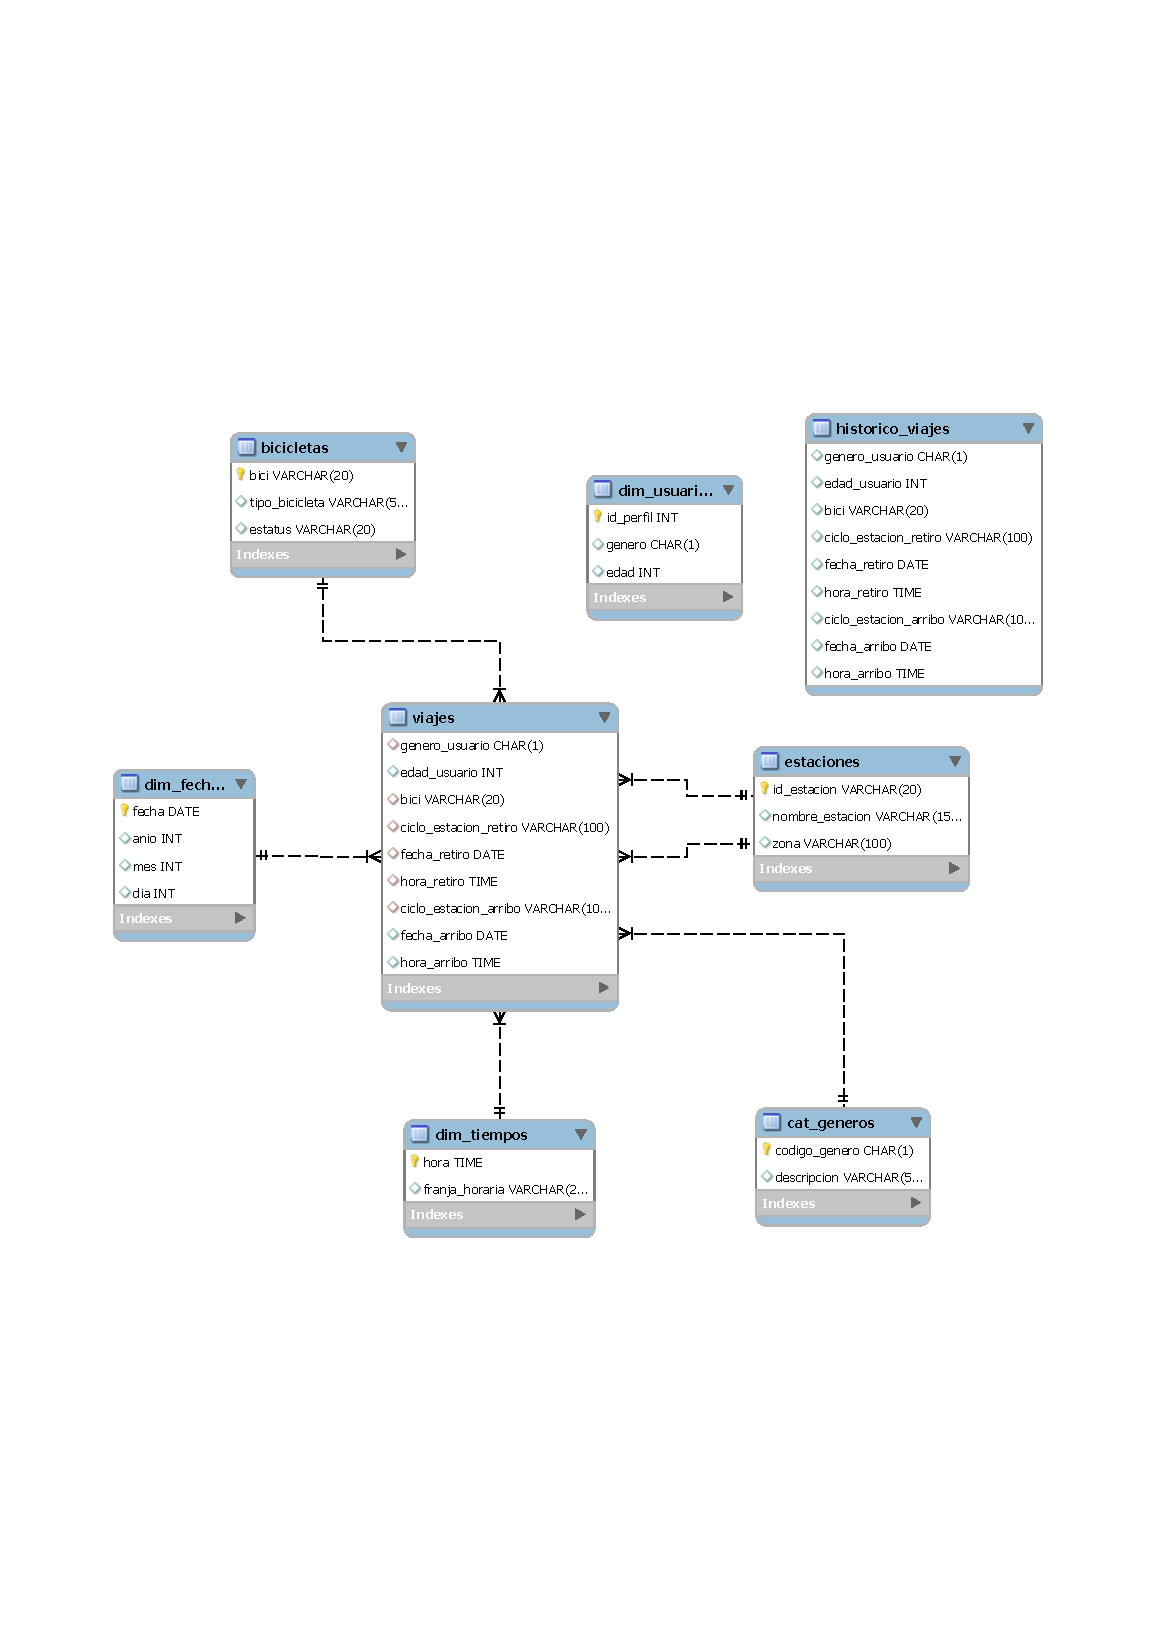
\includegraphics[width=0.8\textwidth]{../Diagrama_EER_Ecobici.pdf}
    \caption{Diagrama Entidad-Relación (Modelo de Estrella) estructurado para el análisis.}
    \label{fig:diagrama_eer}
\end{figure}


\newpage

\section{Enlace a Repositorio GitHub.}

\vspace{5mm}

\begin{center}
    \href{https://github.com/Richard-0x/db-administration}{
        \fbox{\rule{0pt}{12pt}\hspace{8pt}\textbf{Repositorio GitHub}\hspace{8pt}}
    }
\end{center}

\section{Enlace Google Drive}

\vspace{5mm}

\begin{center}
    \href{https://drive.google.com/drive/folders/1ogxHLMOxqbDtDr0JjjXlNfBxNryxPC8Q?usp=sharing}{
        \fbox{\rule{0pt}{12pt}\hspace{8pt}\textbf{DATA DRIVE}\hspace{8pt}}
    }
\end{center}


\end{document}